\documentclass[a4paper]{report} % estilo do documento

\usepackage[utf8]{inputenc} %encoding do ficheiro
\usepackage[portuges]{babel} % para língua portuguesa
\usepackage{graphicx} % para importar imagens

\begin{document}

\title{Relatório Trabalho Prático LI1}
\author{Grupo 00\\
\\
Alan Turing e Edger Dijkstra}
\date{\today}

\maketitle

\tableofcontents

\listoffigures

\listoftables

%% Introdução
\chapter{Introdução}

  \section{Contextualização}
  \ldots

  \section{Motivação}
  \ldots
  
  \section{Objectivos}
  \ldots

%% Análise de Requisitos e Especificação do Problema
\chapter{Análise de Requisitos}


\section{Fase 1}
\label{sec:analisefase1}

Análise sobre o que é pedido na fase 1 do projecto e qual é o problema em concreto.

\ldots

\section{Fase 2}
\label{sec:analisefasee}

Análise sobre o que é pedido na fase 2 do projecto e qual é o problema em concreto.

\ldots


%% Descrição da Solução Desenvolvida
\chapter{A Nossa Solução}
\label{sec:solucao}

Apresentar a solução para os problemas descritos em \ref{sec:analisefase1} e \ref{sec:analisefasee}.

Pode-se inserrir texto a \textbf{negrito} e também a \textit{itálico} \ldots

\begin{enumerate}
\item item 1
\item item 2
\end{enumerate}

Um exemplo em haskell:
\begin{verbatim}
max2 :: Int -> Int -> Int
max2 a b = if a > b then a else b

max3 :: Int -> Int -> Int -> Int
max3 a b c = max2 (max2 a b) c
\end{verbatim}


A tabela \ref{tbl:tabela} apresenta os dados sobre \ldots

\begin{table}[t]
\begin{center}
\begin{tabular}{|c|r||l|}
	\hline
	\emph{Turno} & \textit{Número} & \textbf{Nome}\\
	\hline
	\hline
	PL1 & 1000 & Hugo\\
	PL2 & 2000 & Nuno\\
	\hline
\end{tabular}
\end{center}
\caption{Tabela de turnos.}
\label{tbl:tabela}
\end{table}

\begin{figure}[tb]
\begin{center}
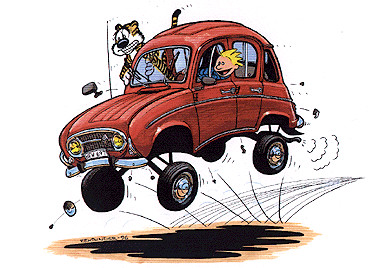
\includegraphics[width=6cm]{calvin.jpg}
\end{center}
\caption{Isto é uma figura.}
\label{manel}
\end{figure}

A formula resolvente é dada na eq. \ref{eq:1} \ldots

\begin{equation}
\label{eq:1}
	x = \frac{-b \pm \sqrt{b^2 - 4ac} }{2a}
\end{equation}

\begin{equation}
\label{eq:2}
	x = \frac{-b \pm \sqrt{b^2 - 4ac}}{2a}
\end{equation}

% Como foi validada a implementação da solução
\chapter{Validação da Solução}

Descrever que abordagem tomaram para validar a solução apresentada na Secção \ref{sec:solucao}.

Em particular pode-se fazer uma descrição dos casos de teste
realizados para validar o desenvolvimento local.


\chapter{Conclusão}

\ldots

\bibliographystyle{plain}
\bibliography{document}    

\end{document}
